%%%%%%%%%%%%%%%%%%%%%%%%%%%%%%%%%%%%%%%%%%%%%%%%%%%%%%%%%%%%%%%%%%%%%%%%%%%%%
% 26/05/2010
% edited by Bill Lampos
%
% Feel free to use (copy) the structure (latex formatting source code)
% but not the content of this document.
%
%%%%%%%%%%%%%%%%%%%%%%%%%%%%%%%%%%%%%%%%%%%%%%%%%%%%%%%%%%%%%%%%%%%%%%%%%%%%%
\documentclass[compress,red]{beamer}
\mode<presentation>

\usetheme{Warsaw}
% other themes: AnnArbor, Antibes, Bergen, Berkeley, Berlin, Boadilla, boxes, CambridgeUS, Copenhagen, Darmstadt, default, Dresden, Frankfurt, Goettingen,
% Hannover, Ilmenau, JuanLesPins, Luebeck, Madrid, Maloe, Marburg, Montpellier, PaloAlto, Pittsburg, Rochester, Singapore, Szeged, classic

%\usecolortheme{lily}
% color themes: albatross, beaver, beetle, crane, default, dolphin, dov, fly, lily, orchid, rose, seagull, seahorse, sidebartab, structure, whale, wolverine

%\usefonttheme{serif}
% font themes: default, professionalfonts, serif, structurebold, structureitalicserif, structuresmallcapsserif

% pdf is displayed in full screen mode automatically
%\hypersetup{pdfpagemode=FullScreen}

% define your own colours:
\definecolor{Red}{rgb}{1,0,0}
\definecolor{Blue}{rgb}{0,0,1}
\definecolor{Green}{rgb}{0,1,0}
\definecolor{magenta}{rgb}{1,0,.6}
\definecolor{lightblue}{rgb}{0,.5,1}
\definecolor{lightpurple}{rgb}{.6,.4,1}
\definecolor{gold}{rgb}{.6,.5,0}
\definecolor{orange}{rgb}{1,0.4,0}
\definecolor{hotpink}{rgb}{1,0,0.5}
\definecolor{newcolor2}{rgb}{.5,.3,.5}
\definecolor{newcolor}{rgb}{0,.3,1}
\definecolor{newcolor3}{rgb}{1,0,.35}
\definecolor{darkgreen1}{rgb}{0, .35, 0}
\definecolor{darkgreen}{rgb}{0, .6, 0}
\definecolor{darkred}{rgb}{.75,0,0}

\xdefinecolor{olive}{cmyk}{0.64,0,0.95,0.4}
\xdefinecolor{purpleish}{cmyk}{0.75,0.75,0,0}

\useoutertheme[subsection=false]{smoothbars}

\usepackage[T1]{fontenc}
\usepackage[utf8]{inputenc}
\usepackage[francais]{babel}

\usepackage{listings}
\usepackage{graphicx}
\usepackage{url}
\usepackage{hyperref}
\usepackage{subfigure}

\newcommand\pro{\item[$+$]}
\newcommand\con{\item[$-$]}

\lstset{
  %backgroundcolor=\color{white},   % choose the background color; you must add \usepackage{color} or \usepackage{xcolor}
  basicstyle=\footnotesize,        % the size of the fonts that are used for the code
  breakatwhitespace=false,         % sets if automatic breaks should only happen at whitespace
  breaklines=true,                 % sets automatic line breaking
  %captionpos=b,                    % sets the caption-position to bottom
  %commentstyle=\color{mygreen},    % comment style
  %deletekeywords={...},            % if you want to delete keywords from the given language
  %escapeinside={\%*}{*)},          % if you want to add LaTeX within your code
  extendedchars=true,              % lets you use non-ASCII characters; for 8-bits encodings only, does not work with UTF-8
  frame=single,	                   % adds a frame around the code
  keepspaces=true,                 % keeps spaces in text, useful for keeping indentation of code (possibly needs columns=flexible)
  %keywordstyle=\color{blue},       % keyword style
  %language=Octave,                 % the language of the code
  %otherkeywords={*,...},           % if you want to add more keywords to the set
  %numbers=left,                    % where to put the line-numbers; possible values are (none, left, right)
  %numbersep=5pt,                   % how far the line-numbers are from the code
  %numberstyle=\tiny\color{mygray}, % the style that is used for the line-numbers
  %rulecolor=\color{black},         % if not set, the frame-color may be changed on line-breaks within not-black text (e.g. comments (green here))
  showspaces=false,                % show spaces everywhere adding particular underscores; it overrides 'showstringspaces'
  showstringspaces=false,          % underline spaces within strings only
  showtabs=false,                  % show tabs within strings adding particular underscores
  stepnumber=2,                    % the step between two line-numbers. If it's 1, each line will be numbered
  %stringstyle=\color{mymauve},     % string literal style
  tabsize=2,	                   % sets default tabsize to 2 spaces
  %title=\lstname                   % show the filename of files included with \lstinputlisting; also try caption instead of title
}

\title{Déboguage de code natif OCaml sous LLDB}
\subtitle{Master 2 STL - Soutenance de stage}
\author{Elias Boutaleb}
\institute{OCamlPro}
\date{\today}

\AtBeginSection[]
{
    \begin{frame}
     \tableofcontents[currentsection]
    \end{frame}
}

\begin{document}

\frame{
	\titlepage
}

% le contenu de la presentation va etre dense
%je coupe la partie sur la societe
\frame{\tableofcontents}

\section{Introduction}
\subsection{Pourquoi?}

\frame{\frametitle{Pourquoi?}

\vspace{0.25cm}

Pourquoi déboguer du code natif? \pause

\begin{itemize}
\item Besoin de déboguer du code optimisé
%un bug peut apparaitre dans du code optimisé qui n'apparait pas dans sa version non optimisé
\item Il n'y a pas encore de solution définitive pour déboguer du code natif OCaml
% patchs, outils qui restent incomplets, limités, dispersés et non disponible au public
\item Besoin d'un débogueur au niveau de la source
% tous les devs ne peuvent pas forcement lire l'asm,  et parmi ceux qui peuvent,
    % doit garder en tete du contexte sur l'archi
    % utilisee et le runtime OCaml, en plus de cleui du programme
\end{itemize}
\vspace{0.25cm}

Pourquoi sous LLDB? \pause

\vspace{0.25cm}
\begin{itemize}
\item Support d'OCaml inexistant
%lldb ne sait meme pas qu'il debugge un binaire OCaml
% MS s'occupe deja du support cote gdb
\item ocplib-lldb : une liaison (binding) vers lldb en OCaml
% pour profiter de cette lib
%gen auto de liaison faite en parsant les entetes C++ de LLDB
%\item Apple préfere LLVM à la toolchain GNU
%(XCode utilise LLDB pour deboguer du ObjC et Swift)
\end{itemize}
}

\frame{\frametitle{Choses à savoir concernant le code natif}
\begin{itemize}
    \item Le code machine ne conserve aucune abstraction
        %presentes dans le code source, ni dans l'AST, les IRs, aucun type
    \item Les optimisations peuvent transformer le programme
        % plus difficile d'etablir correspondance entre une construction
        % syntaxique dans le language source , ses IR et un ensemble d'ins en code natif
    %\item Tout cela implique des pertes d'information
\end{itemize}
}

\subsection{A l'heure actuelle}
\frame{\frametitle{A l'heure actuelle}
Il y a un support partiel pour le déboguage natif de code OCaml.

\begin{itemize}
    \item Consultation de la pile d'appels de fonction
        %directives DWARF CFI permettent de la reconstruire
    \item Pas à pas partiel aux points d'entrée et d'appel de fonction
        %consequence du patch de thomasg qui propage les debug events du BC vers le backend natif
    \item Profilage mémoire de programmes OCaml
        % pour pister consommation memoire des progs, pour pouv permettre collection de ces infos, modification des entetes des blocs memoire
        % dans memprof - compil fork par ocamlpro  fait adjonction d'identifiants de location (type + place dans la source) depuis le compilateur
        % possible d'interpreter val selon type et emplacement dans la source, quand cette valeur est encore vivante dans le tas
\end{itemize}
}

\subsection{Objectifs du stage}
\frame{\frametitle{Objectifs du stage}

% améliorer l'experience de debug sous LLDB en general
\begin{enumerate}
    \item Modifier le compilateur pour générer plus d'informations de déboguage
        % emplacement des variables en memoire, ameliroer le pas a pas dans la
        % source
    \item Améliorer le prototype de débogueur natif OCaml ocp-lldb
    % basé sur les bindings générés par ocplib-lldb
        % en utilisant les infos generes depuis le compilateur
        % affichage des valeurs de variables, pas a pas dans la source, placer points d'arret aux fcts et fichier/ligne
\end{enumerate}
}

\section{DWARF}

%transition
%pour pouvoir etablir correspondance entre source et code machine, on veut pouvoir
% - collecter toutes les infos generees dans la transformation du code source passe a un compilateur
% - representer ces donnees dans un format adequat, de maniere concise et compacte, et suffisamment de details

\subsection{Présentation de DWARF}
\frame{\frametitle{Présentation de DWARF (1)}

\begin{columns}
    \begin{column}{0.48\textwidth}
        \centering
        
\includegraphics[width=0.5\textwidth]{dwarf.png}%
    \end{column}
    \begin{column}{0.48\textwidth}
        \centering
        
\includegraphics[width=0.5\textwidth]{df2.png}
    \end{column}
\end{columns}

\begin{itemize}
\item Format d'informations de déboguage
%les stocke, largement utilise aujourdhui
\item Indépendant du language de programmation
% peut representer et exprimer multitude de lang HL
% C/Cpp/fortran/go/java
\item Indépendant du compilateur/assembleur/debogueur
%gcc/clang, gdb/lldb
% fichier objet = code + metadonnees pour linking/debug/profile/stack unwind/relocation
\item (Semi-)indépendant du format de fichier objet
 %(même si utilisé le plus souvent en complement avec le format ELF)
\item Standardisé et extensible
% un comité recueille propositions d'extensions du std, suit evol des
    % fonctionalites et des PLs,
\end{itemize}
}

\frame{\frametitle{Présentation de DWARF (2)}

Chaque type de données est placé dans une section dédiée dans le binaire.

%je passe sur la repr binaire du format dwarf
%j'expose ici les sections DWARF les plus importantes pour un debogueur

\begin{itemize}
\item .debug\_info: contient les informations principales DWARF
%\item .debug\_abbrev: "abbréviations" (signatures d'entrées) utilisées pour décoder .debug\_info
% decrivent forme des records utilises dans debug_info
\item .debug\_loc: listes de locations (emplacement des variables à l'exécution)
% sur la pile (et dans le cas, quel offset),  dans un registre
\item .debug\_line: table des numéros de ligne dans la source
% etablit correspondance entre adresses memoires du code executable et les lignes du code source
\end{itemize}
}

\frame{\frametitle{Une section importante : .debug\_info}

\begin{itemize}
\item Entité de base : le DIE (Debugging Information Entry)
%entree d'info de debug : enregistrement
\item DIE = un tag + ensemble d'attributs
\item Un tag spécifie ce que le DIE represente (variable, portée lexicale, fonction, type)
% quel construct est représenté ici

\item Un attribut = couple de clé/valeur
%(fst décrit ce qui est repr - un nom, une adresse, snd une valeur (peut etre un nombre, offset, adresse, chaine, bool)
\item Peut réferencer d'autres entrées, voire d'autres sections

\item Les DIES peuvent etre imbriqués dans d'autres DIES, formant une structure d'arbre
\item Une unité de compilation (CU) <=> un fichier source compilé /objet
    % c'est aussi une entree qui constitue la racine
%\item Compilation séparée : mise en commun des sections DWARF dans des sections communes au binaire final (linker)

\end{itemize}
}


\subsection{Exemple}
\frame{\frametitle{Exemple}
\lstinputlisting[language=C, firstline=3, lastline=14]{d.c}
}

\frame{\frametitle{Arbre d'entrées}
\centering
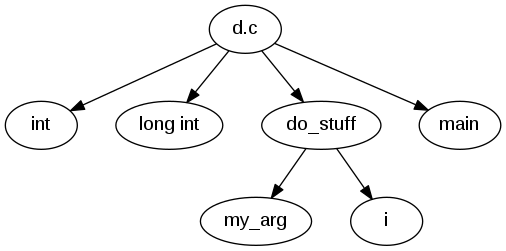
\includegraphics[width=0.85\textwidth]{test.png}
}

\frame{\frametitle{Exemple (2)}
\lstinputlisting[firstline=11, lastline=18]{dwarf}
}

\frame{\frametitle{Exemple (3)}
\lstinputlisting[firstline=43, lastline=50]{dwarf}
}

\frame{\frametitle{Exemple (4)}
\lstinputlisting[firstline=59, lastline=69]{dwarf}
}

% call_frame_cfa : retrieve cfa frame base location from debug_frame section
\frame{\frametitle{Exemple (5)}
\lstinputlisting[firstline=70, lastline=82]{dwarf}
}

% vous pouvez voir que ce format n'est pas sense etre lu par des humains

\subsection{ocplib-dwarf}
\frame{\frametitle{ocplib-dwarf}
\begin{itemize}
\item Bibliothèque de lecture et d'affichage d'informations DWARF
%sortie similaire a objdump
\item Offre une abstraction permettant de manipuler les structures de données
    % utilise des zippers de forets (Gerard Huet) dont chaque noeud contine une liste de sous
    % arbres - acces constant amorti en moyenne
\item Ecriture et édition restent à faire
% meme si cette tache est deleguee aux compilateurs
\end{itemize}
}

%transition : le format dwarf semble ideal pour stocker les infos de debug
%sa complexite est telle qu'il peut decrire du C++

\section{Ajouts faits au compilateur natif}
\subsection{Propagation des évenements de déboguage}
\frame{\frametitle{Propagation des évenements de déboguage (1)}
    \begin{itemize}
\item On veut améliorer le pas à pas dans le code source
    % pas seulement aux appels de fonctions, mais aussi dans des assignations
    % (ref mutables ou pas), branches
\item Nécessaire pour poser des points d'arrêt suivant fichier et numéro de ligne
\item Comment?
    \begin{itemize}
        \item Dans le code assembleur, présence de directives .loc
    \end{itemize}
    %fichier - num de ligne - num de colonne
    %assembleur recupere les infos et l'offset et encode tout cela dans une structure dediée dans la section .debug\_line

\end{itemize}
}

\frame{\frametitle{Propagation des évenements de déboguage (2)}
\begin{itemize}
\item Le bytecode OCaml contient des évenements de déboguage
    %(info de num de ligne/colonne/fichier)
\item Idée : propager ces informations à travers le backend
% patch de tg porte de 3.12.1 a 4.02.1
% emballer chaque noeud des IRs dans un enregistrement polymorphique avec un
    % champ d'info de ligne
\item Affecte les assignations non-constantes, les entiers et certaines primitives
% assignation, comparaisons lors de test, allocation

\item Inconvénients :
\begin{enumerate}
\con Modifications lourdes du compilateur
% languages des passes backend natif n'a pas prevu pour l'adjonction d'info de debug
\con Manque de précision, perte d'informations
% code subit encore des transformations/optimisations, est expansé puis réduit
% csq du manque de precision
\end{enumerate}

\end{itemize}
}

\subsection{Accès aux variables à l'éxecution}
\frame{\frametitle{Accès aux variables à l'éxecution}
\begin{itemize}
\item Deux passes supplémentaires dans le backend: available\_regs et available\_ranges
% emploie tech d'analyse de flot de donnees en avant
% available\_regs parcourt le CFG Mach d'une fonction et determine pour chaque ins manip/l'ins courante  l'ens des regs avec un ident "disponibles",
%cad dont la valeur peut etre inspectee par un debuggeur
% available_ranges determine pour chaque variable/identifieur d'une fonction les intervalles ou son contenu est disponible,
% et pour chaque intervalle, le registre qui contient cette valeur
\item Ne capturent pas les variables victimes d'optimisations
% cst folding - reduction de constantes
% Mark veut y remedier avec des let fantomes dans flambda
\item Un emetteur DWARF peuple les sections .debug\_info et .debug\_loc
\item Valeurs disponibles pas toujours cohérentes
\item Fourni et développé par Mark Shinwell (Jane Street)
%id unique conservé en cas de masquage de variable
\end{itemize}
}

\subsection{Informations de type}
\frame{\frametitle{Informations de type}
\begin{itemize}
    \item L'arbre syntaxique typé peut être sérialisé dans un fichier .cmt\\
    \item Ecriture dans le binaire en tant que symbole
\end{itemize}

%\begin{itemize}
%\pro Plus pratique que de manipuler les fichiers .cmt
%\con Taille plus importante du binaire
%\con Nécessite modification du compilateur
%\end{itemize}
}

\section{Déboguage sous LLDB}
\subsection{Plugin LLDB pour OCaml}
\frame{\frametitle{Plugin LLDB pour OCaml (1)}
\begin{itemize}
\item A ce stade, le binaire contient plus d'informations... \pause
%plus d'endroits ou poser un point d'arrêt
\item ...qui ne peuvent pas être lues par LLDB \pause
% DWARF emis pas structure comme celui de C/C++, et
% LLDB croit qu'il debugge du C
\item Maintenant possible d'ajouter d'autres languages à LLDB
% depuis un an, chgmts faits a LLDB pour pouvoir supporter d'autres languages que ceux supportes par clang
% il suffit d'ecrire des classes impl certaines interfaces
% ajouter le language cible dans un enum
% eventuellement pouvoir evaluer expr dans ce language
% pretty printing des valeurs et typage dynamique, ptes statiques ou dyn du language
\end{itemize}
}

\frame{\frametitle{Plugin LLDB pour OCaml (2) - Contenu}
\begin{itemize}
\item Un parseur d'informations DWARF personalisé
\item Un système de type minimal
%(toutes les valeurs sont des entiers 64 bits, leur eval est laissee a ocp-lldb)
\item Supporte le démanglage des symboles
\end{itemize}
}

\subsection{Ajouts faits à ocp-lldb}

\frame{\frametitle{Ajouts faits à ocp-lldb}
La bibliothèque ocplib-lldb \\

\begin{itemize}
    \item Tire profit du front-end OCaml
    %structure des noeuds de l'ast/typedtree, types peuvent changer d'une version du compilateur a une autre
    % debat selon cmt/types dans le dwarf, mais changements dans couche de debug dediee ocaml plus facile et maintenable que de modifier le compilateur
    \item Peut générer une liaison avec l'API de LLDB en OCaml
    % parsant les entetes C++ definissant lAPI de la librarie liblldb qui
    % permet de commander instances de lldb via liblldb
    % majeure partie des enums et de l'API supportes, fonction statiques nope
    % acces aux objets se fait via la FFI
\end{itemize}

Le débogueur ocp-lldb
\begin{itemize}
\item Une table de symboles est construite à partir de l'arbre syntaxique typé
% lit le typedtree serialise dans le binaire, l'explore et en extrait une structure d'arbre plus simple et compacte
\item Peut récuperer le type associé à un identifiant et afficher sa valeur
\end{itemize}

}


\frame{\frametitle{Démonstration}
}


% amelioration
%commande qui liste les endroits ou un bp peut etre place?

\section*{Conclusion}

\frame{\frametitle{Conclusion}

Etat actuel du projet

\begin{itemize}
\item Systèmes visés pour l'instant : Linux x86 64 bits
\item Modifications du compilateur bientôt disponible au public
% dans un futur plus ou moins proche
\item Emission DWARF
\footnote{\url{https://github.com/ocaml/ocaml/pull/574}}
%de MS et deboguage natif: peut etre pour 4.05
% amelioration faites depuis 4.02 concernent surtout flambda et gdb
\item Le plugin LLDB pour OCaml a intégré LLDB
% il reste encore deux patchs a integrer
% cela reste en suspend, demanglage dependra de comment MS veut implanter cela
\item ocp-lldb et ocp-dwarf sont disponibles
    %mais necessite mes modifs
\end{itemize}

Difficultés

\begin{itemize}
\item Augmenter le nombre d'évenements de déboguage
\item Améliorer leur précision
% chronophage car precision de methode naive + temps de compilation de la compiler suite
% comment faire composer les differents constructs ensemble
% insertion des events, mais le code/IR subit encore des transformations
% Modifications entre debugger et compiler
\end{itemize}
}

\frame{\frametitle{Fin}
    \begin{center}
        \huge Merci de votre attention! \\
        \vspace{0.25cm}
        \huge Avez-vous des questions?
    \end{center}
}

\end{document}
